\documentclass{extbook}[14pt]
\usepackage{multicol, enumerate, enumitem, hyperref, color, soul, setspace, parskip, fancyhdr, amssymb, amsthm, amsmath, latexsym, units, mathtools}
\everymath{\displaystyle}
\usepackage[headsep=0.5cm,headheight=0cm, left=1 in,right= 1 in,top= 1 in,bottom= 1 in]{geometry}
\usepackage{dashrule}  % Package to use the command below to create lines between items
\newcommand{\litem}[1]{\item #1

\rule{\textwidth}{0.4pt}}
\pagestyle{fancy}
\lhead{}
\chead{Answer Key for Progress Quiz 6 Version B}
\rhead{}
\lfoot{4563-7456}
\cfoot{}
\rfoot{Summer C 2021}
\begin{document}
\textbf{This key should allow you to understand why you choose the option you did (beyond just getting a question right or wrong). \href{https://xronos.clas.ufl.edu/mac1105spring2020/courseDescriptionAndMisc/Exams/LearningFromResults}{More instructions on how to use this key can be found here}.}

\textbf{If you have a suggestion to make the keys better, \href{https://forms.gle/CZkbZmPbC9XALEE88}{please fill out the short survey here}.}

\textit{Note: This key is auto-generated and may contain issues and/or errors. The keys are reviewed after each exam to ensure grading is done accurately. If there are issues (like duplicate options), they are noted in the offline gradebook. The keys are a work-in-progress to give students as many resources to improve as possible.}

\rule{\textwidth}{0.4pt}

\begin{enumerate}\litem{
Construct the lowest-degree polynomial given the zeros below. Then, choose the intervals that contain the coefficients of the polynomial in the form $x^3+bx^2+cx+d$.
\[ -5 + 5 i \text{ and } 3 \]The solution is \( x^{3} +7 x^{2} +20 x -150 \), which is option C.\begin{enumerate}[label=\Alph*.]
\item \( b \in [-11, -3], c \in [16, 22], \text{ and } d \in [145, 151] \)

$x^{3} -7 x^{2} +20 x + 150$, which corresponds to multiplying out $(x-(-5 + 5 i))(x-(-5 - 5 i))(x + 3)$.
\item \( b \in [1, 6], c \in [-1, 7], \text{ and } d \in [-18, -13] \)

$x^{3} + x^{2} +2 x -15$, which corresponds to multiplying out $(x + 5)(x -3)$.
\item \( b \in [2, 12], c \in [16, 22], \text{ and } d \in [-156, -141] \)

* $x^{3} +7 x^{2} +20 x -150$, which is the correct option.
\item \( b \in [1, 6], c \in [-9, 1], \text{ and } d \in [13, 20] \)

$x^{3} + x^{2} -8 x + 15$, which corresponds to multiplying out $(x -5)(x -3)$.
\item \( \text{None of the above.} \)

This corresponds to making an unanticipated error or not understanding how to use nonreal complex numbers to create the lowest-degree polynomial. If you chose this and are not sure what you did wrong, please contact the coordinator for help.
\end{enumerate}

\textbf{General Comment:} Remember that the conjugate of $a+bi$ is $a-bi$. Since these zeros always come in pairs, we need to multiply out $(x-(-5 + 5 i))(x-(-5 - 5 i))(x-(3))$.
}
\litem{
Which of the following equations \textit{could} be of the graph presented below?

\begin{center}
    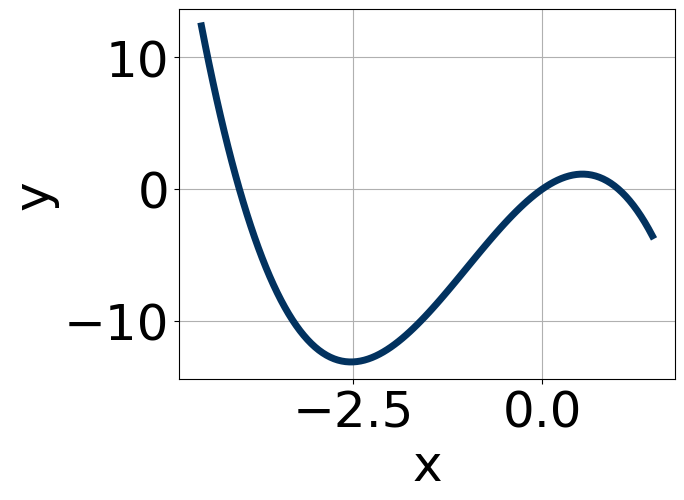
\includegraphics[width=0.5\textwidth]{../Figures/polyGraphToFunctionB.png}
\end{center}


The solution is \( -9x^{5} (x - 1)^{9} (x + 4)^{9} \), which is option A.\begin{enumerate}[label=\Alph*.]
\item \( -9x^{5} (x - 1)^{9} (x + 4)^{9} \)

* This is the correct option.
\item \( 17x^{11} (x - 1)^{9} (x + 4)^{9} \)

This corresponds to the leading coefficient being the opposite value than it should be.
\item \( 6x^{5} (x - 1)^{8} (x + 4)^{9} \)

The factor $(x - 1)$ should have an odd power and the leading coefficient should be the opposite sign.
\item \( -7x^{7} (x - 1)^{8} (x + 4)^{4} \)

The factors $1$ and $-4$ have have been odd power.
\item \( -17x^{7} (x - 1)^{10} (x + 4)^{9} \)

The factor $1$ should have been an odd power.
\end{enumerate}

\textbf{General Comment:} General Comments: Draw the x-axis to determine which zeros are touching (and so have even multiplicity) or cross (and have odd multiplicity).
}
\litem{
Which of the following equations \textit{could} be of the graph presented below?

\begin{center}
    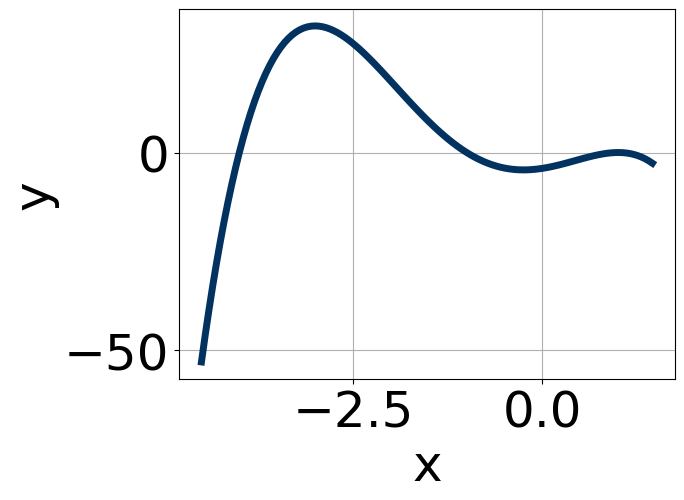
\includegraphics[width=0.5\textwidth]{../Figures/polyGraphToFunctionCopyB.png}
\end{center}


The solution is \( -4(x - 1)^{10} (x + 4)^{7} (x + 1)^{9} \), which is option E.\begin{enumerate}[label=\Alph*.]
\item \( -17(x - 1)^{4} (x + 4)^{8} (x + 1)^{9} \)

The factor $(x + 4)$ should have an odd power.
\item \( 20(x - 1)^{10} (x + 4)^{7} (x + 1)^{4} \)

The factor $(x + 1)$ should have an odd power and the leading coefficient should be the opposite sign.
\item \( 2(x - 1)^{10} (x + 4)^{9} (x + 1)^{9} \)

This corresponds to the leading coefficient being the opposite value than it should be.
\item \( -6(x - 1)^{7} (x + 4)^{8} (x + 1)^{11} \)

The factor $1$ should have an even power and the factor $-4$ should have an odd power.
\item \( -4(x - 1)^{10} (x + 4)^{7} (x + 1)^{9} \)

* This is the correct option.
\end{enumerate}

\textbf{General Comment:} General Comments: Draw the x-axis to determine which zeros are touching (and so have even multiplicity) or cross (and have odd multiplicity).
}
\litem{
Describe the zero behavior of the zero $x = -6$ of the polynomial below.
\[ f(x) = -4(x - 8)^{6}(x + 8)^{2}(x + 6)^{9}(x - 6)^{6} \]The solution is the graph below, which is option A.
    \begin{center}
        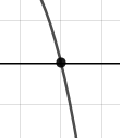
\includegraphics[width=0.3\textwidth]{../Figures/polyZeroBehaviorCopyAB.png}
    \end{center}\begin{enumerate}[label=\Alph*.]
\begin{multicols}{2}
\item 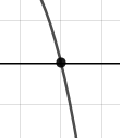
\includegraphics[width = 0.3\textwidth]{../Figures/polyZeroBehaviorCopyAB.png}
\item 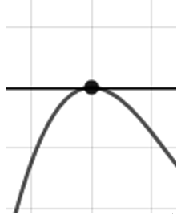
\includegraphics[width = 0.3\textwidth]{../Figures/polyZeroBehaviorCopyBB.png}
\item 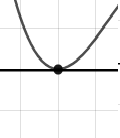
\includegraphics[width = 0.3\textwidth]{../Figures/polyZeroBehaviorCopyCB.png}
\item 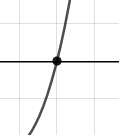
\includegraphics[width = 0.3\textwidth]{../Figures/polyZeroBehaviorCopyDB.png}
\end{multicols}\item None of the above.\end{enumerate}
\textbf{General Comment:} You will need to sketch the entire graph, then zoom in on the zero the question asks about.
}
\litem{
Construct the lowest-degree polynomial given the zeros below. Then, choose the intervals that contain the coefficients of the polynomial in the form $x^3+bx^2+cx+d$.
\[ -4 - 2 i \text{ and } -2 \]The solution is \( x^{3} +10 x^{2} +36 x + 40 \), which is option A.\begin{enumerate}[label=\Alph*.]
\item \( b \in [8, 13], c \in [34.2, 37], \text{ and } d \in [40, 42] \)

* $x^{3} +10 x^{2} +36 x + 40$, which is the correct option.
\item \( b \in [-4, 6], c \in [4.5, 8.2], \text{ and } d \in [6, 9] \)

$x^{3} + x^{2} +6 x + 8$, which corresponds to multiplying out $(x + 4)(x + 2)$.
\item \( b \in [-4, 6], c \in [3, 4.3], \text{ and } d \in [2, 5] \)

$x^{3} + x^{2} +4 x + 4$, which corresponds to multiplying out $(x + 2)(x + 2)$.
\item \( b \in [-14, -8], c \in [34.2, 37], \text{ and } d \in [-40, -32] \)

$x^{3} -10 x^{2} +36 x -40$, which corresponds to multiplying out $(x-(-4 - 2 i))(x-(-4 + 2 i))(x -2)$.
\item \( \text{None of the above.} \)

This corresponds to making an unanticipated error or not understanding how to use nonreal complex numbers to create the lowest-degree polynomial. If you chose this and are not sure what you did wrong, please contact the coordinator for help.
\end{enumerate}

\textbf{General Comment:} Remember that the conjugate of $a+bi$ is $a-bi$. Since these zeros always come in pairs, we need to multiply out $(x-(-4 - 2 i))(x-(-4 + 2 i))(x-(-2))$.
}
\litem{
Construct the lowest-degree polynomial given the zeros below. Then, choose the intervals that contain the coefficients of the polynomial in the form $ax^3+bx^2+cx+d$.
\[ \frac{-7}{5}, \frac{5}{2}, \text{ and } \frac{-1}{4} \]The solution is \( 40x^{3} -34 x^{2} -151 x -35 \), which is option D.\begin{enumerate}[label=\Alph*.]
\item \( a \in [35, 41], b \in [48, 58], c \in [-131, -125], \text{ and } d \in [-42, -32] \)

$40x^{3} +54 x^{2} -129 x -35$, which corresponds to multiplying out $(5x -7)(2x + 5)(4x + 1)$.
\item \( a \in [35, 41], b \in [-36, -27], c \in [-158, -150], \text{ and } d \in [33, 37] \)

$40x^{3} -34 x^{2} -151 x + 35$, which corresponds to multiplying everything correctly except the constant term.
\item \( a \in [35, 41], b \in [-148, -145], c \in [95, 106], \text{ and } d \in [33, 37] \)

$40x^{3} -146 x^{2} +101 x + 35$, which corresponds to multiplying out $(5x -7)(2x -5)(4x + 1)$.
\item \( a \in [35, 41], b \in [-36, -27], c \in [-158, -150], \text{ and } d \in [-42, -32] \)

* $40x^{3} -34 x^{2} -151 x -35$, which is the correct option.
\item \( a \in [35, 41], b \in [32, 40], c \in [-158, -150], \text{ and } d \in [33, 37] \)

$40x^{3} +34 x^{2} -151 x + 35$, which corresponds to multiplying out $(5x -7)(2x + 5)(4x -1)$.
\end{enumerate}

\textbf{General Comment:} To construct the lowest-degree polynomial, you want to multiply out $(5x + 7)(2x -5)(4x + 1)$
}
\litem{
Describe the end behavior of the polynomial below.
\[ f(x) = 8(x - 4)^{4}(x + 4)^{9}(x + 8)^{4}(x - 8)^{5} \]The solution is the graph below, which is option C.
    \begin{center}
        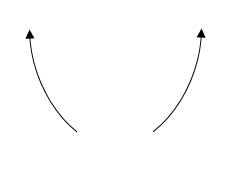
\includegraphics[width=0.3\textwidth]{../Figures/polyEndBehaviorCB.png}
    \end{center}\begin{enumerate}[label=\Alph*.]
\begin{multicols}{2}
\item 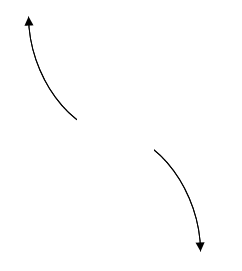
\includegraphics[width = 0.3\textwidth]{../Figures/polyEndBehaviorAB.png}
\item 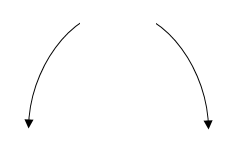
\includegraphics[width = 0.3\textwidth]{../Figures/polyEndBehaviorBB.png}
\item 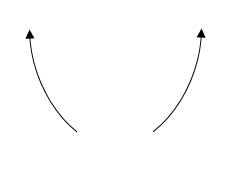
\includegraphics[width = 0.3\textwidth]{../Figures/polyEndBehaviorCB.png}
\item 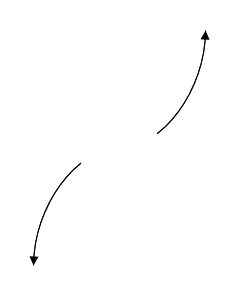
\includegraphics[width = 0.3\textwidth]{../Figures/polyEndBehaviorDB.png}
\end{multicols}\item None of the above.\end{enumerate}
\textbf{General Comment:} Remember that end behavior is determined by the leading coefficient AND whether the \textbf{sum} of the multiplicities is positive or negative.
}
\litem{
Construct the lowest-degree polynomial given the zeros below. Then, choose the intervals that contain the coefficients of the polynomial in the form $ax^3+bx^2+cx+d$.
\[ \frac{1}{2}, \frac{7}{4}, \text{ and } 4 \]The solution is \( 8x^{3} -50 x^{2} +79 x -28 \), which is option B.\begin{enumerate}[label=\Alph*.]
\item \( a \in [7, 12], b \in [-23, -12], c \in [-71, -59], \text{ and } d \in [-32, -21] \)

$8x^{3} -14 x^{2} -65 x -28$, which corresponds to multiplying out $(2x + 1)(4x + 7)(x -4)$.
\item \( a \in [7, 12], b \in [-51, -44], c \in [77, 82], \text{ and } d \in [-32, -21] \)

* $8x^{3} -50 x^{2} +79 x -28$, which is the correct option.
\item \( a \in [7, 12], b \in [49, 55], c \in [77, 82], \text{ and } d \in [28, 30] \)

$8x^{3} +50 x^{2} +79 x + 28$, which corresponds to multiplying out $(2x + 1)(4x + 7)(x + 4)$.
\item \( a \in [7, 12], b \in [-51, -44], c \in [77, 82], \text{ and } d \in [28, 30] \)

$8x^{3} -50 x^{2} +79 x + 28$, which corresponds to multiplying everything correctly except the constant term.
\item \( a \in [7, 12], b \in [-44, -34], c \in [31, 43], \text{ and } d \in [28, 30] \)

$8x^{3} -42 x^{2} +33 x + 28$, which corresponds to multiplying out $(2x + 1)(4x -7)(x -4)$.
\end{enumerate}

\textbf{General Comment:} To construct the lowest-degree polynomial, you want to multiply out $(2x -1)(4x -7)(x -4)$
}
\litem{
Describe the zero behavior of the zero $x = 2$ of the polynomial below.
\[ f(x) = -4(x - 2)^{5}(x + 2)^{10}(x - 3)^{6}(x + 3)^{10} \]The solution is the graph below, which is option A.
    \begin{center}
        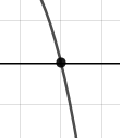
\includegraphics[width=0.3\textwidth]{../Figures/polyZeroBehaviorAB.png}
    \end{center}\begin{enumerate}[label=\Alph*.]
\begin{multicols}{2}
\item 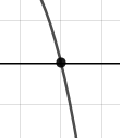
\includegraphics[width = 0.3\textwidth]{../Figures/polyZeroBehaviorAB.png}
\item 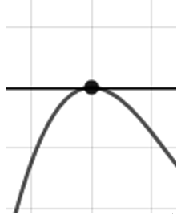
\includegraphics[width = 0.3\textwidth]{../Figures/polyZeroBehaviorBB.png}
\item 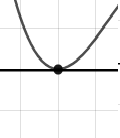
\includegraphics[width = 0.3\textwidth]{../Figures/polyZeroBehaviorCB.png}
\item 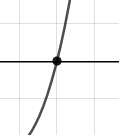
\includegraphics[width = 0.3\textwidth]{../Figures/polyZeroBehaviorDB.png}
\end{multicols}\item None of the above.\end{enumerate}
\textbf{General Comment:} You will need to sketch the entire graph, then zoom in on the zero the question asks about.
}
\litem{
Describe the end behavior of the polynomial below.
\[ f(x) = 2(x + 5)^{3}(x - 5)^{6}(x + 3)^{3}(x - 3)^{5} \]The solution is the graph below, which is option D.
    \begin{center}
        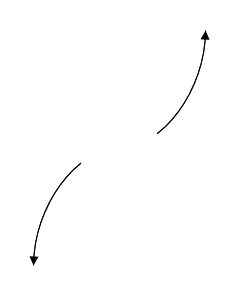
\includegraphics[width=0.3\textwidth]{../Figures/polyEndBehaviorCopyDB.png}
    \end{center}\begin{enumerate}[label=\Alph*.]
\begin{multicols}{2}
\item 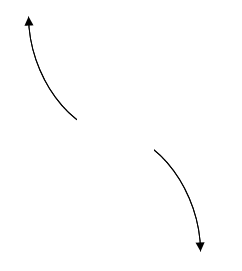
\includegraphics[width = 0.3\textwidth]{../Figures/polyEndBehaviorCopyAB.png}
\item 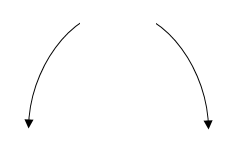
\includegraphics[width = 0.3\textwidth]{../Figures/polyEndBehaviorCopyBB.png}
\item 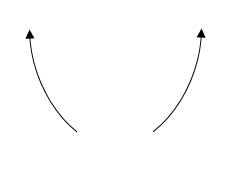
\includegraphics[width = 0.3\textwidth]{../Figures/polyEndBehaviorCopyCB.png}
\item 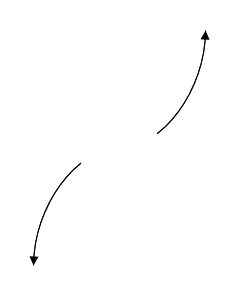
\includegraphics[width = 0.3\textwidth]{../Figures/polyEndBehaviorCopyDB.png}
\end{multicols}\item None of the above.\end{enumerate}
\textbf{General Comment:} Remember that end behavior is determined by the leading coefficient AND whether the \textbf{sum} of the multiplicities is positive or negative.
}
\end{enumerate}

\end{document}